\documentclass{article}

% Language setting
\usepackage[english]{babel}

% Set page size and margins
\usepackage[letterpaper,top=2cm,bottom=2cm,left=3cm,right=3cm,marginparwidth=1.75cm]{geometry}

% Useful packages
\usepackage{amsmath}
\usepackage{amssymb}
\usepackage{graphicx}
\usepackage[colorlinks=true, allcolors=blue]{hyperref}
\usepackage{float}
\usepackage{url}
\usepackage{cite}
\usepackage{enumitem}
\usepackage{tikz}
\setlength{\parskip}{0.5em}

\title{Root Test of Factorial and Beyond}
\author{Yicheng (Eason) Jiang}

\begin{document}
\maketitle

\begin{abstract}
This article extends the regular college level calculus II into a higher level by putting root test in a series with factorial, and furthermore study about the nth root of factorial ($\sqrt[n]{n!}$). By studying this specific limit ($ \displaystyle \lim_{n \to \infty }\frac{\sqrt[n]{n!}}{n}$), we found that there is some connections between the nth root of factorial and The Optimal Stopping Problem. Also, by comparing the root test and ratio test, we've also found some interesting connections between those. 
\end{abstract}

\section{Introduction}
First, I want to introduce the question that inspired me:
\begin{equation}
\sum_{n=1}^{\infty} \frac{n!}{n^n}
\end{equation}
And we want to show whether this is convergent. Regularly, we can use the Ratio Test, because obviously there is a factorial.
\begin{align}
L_{\text{Ratio}} &= \lim_{n \to \infty} \left| \frac{a_{n+1}}{a_n} \right| \nonumber \\
  &= \lim_{n \to \infty} \frac{(n+1)!}{(n+1)^{n+1}} \cdot \frac{n^n}{n!} \nonumber \\
  &= \lim_{n \to \infty} \frac{(n+1) \cdot n! \cdot n^n}{(n+1) \cdot (n+1)^n \cdot n!} \nonumber \\
  &= \lim_{n \to \infty} \frac{n^n}{(n+1)^n} \nonumber \\
  &= \lim_{n \to \infty} \left( \frac{n}{n+1} \right)^n \nonumber \\
  &= \lim_{n \to \infty} \left( \frac{n+1-1}{n+1} \right)^n \nonumber \\
  &= \lim_{n \to \infty} \left( 1-\frac{1}{n+1} \right)^n 
\end{align}
From here, we can see that the limit is similar to the definition of e, and this types of limit is actually $e^a$. The reader may easily prove the limit is 1/e.
\begin{equation}
 L_{\text{Ratio}} = \lim_{n \to \infty} \left( 1+\frac{-1}{n+1} \right)^n = e^{-1} =\frac{1}{e}<1
\end{equation}
So we've showed that by Ratio Test, the series converges. But this is not fun, because it's just a regular calculus II question. Now, let's try using root test to do the same thing, because there is a $n^n$.
\begin{align}
L_{\text{Root}} &= \lim_{n \to \infty} \sqrt[n]{a_n} \nonumber \\
&= \lim_{n \to \infty} \sqrt[n]{\frac{n!}{n^n}} \nonumber\\
&= \lim_{n \to \infty} \frac{\sqrt[n]{n!}}{n}
\label{eq:one_over_e_limit}
\end{align}
This limit is very important, and our topic is going to extend by this limit. Now, the problem here is the nth root of factorial can't be simplified easily. So I am going to use the numerical method to solve it. If you want to see the proof, please go Appendix A, the proof was really beautiful. 
\begin{figure}[H]
    \centering
    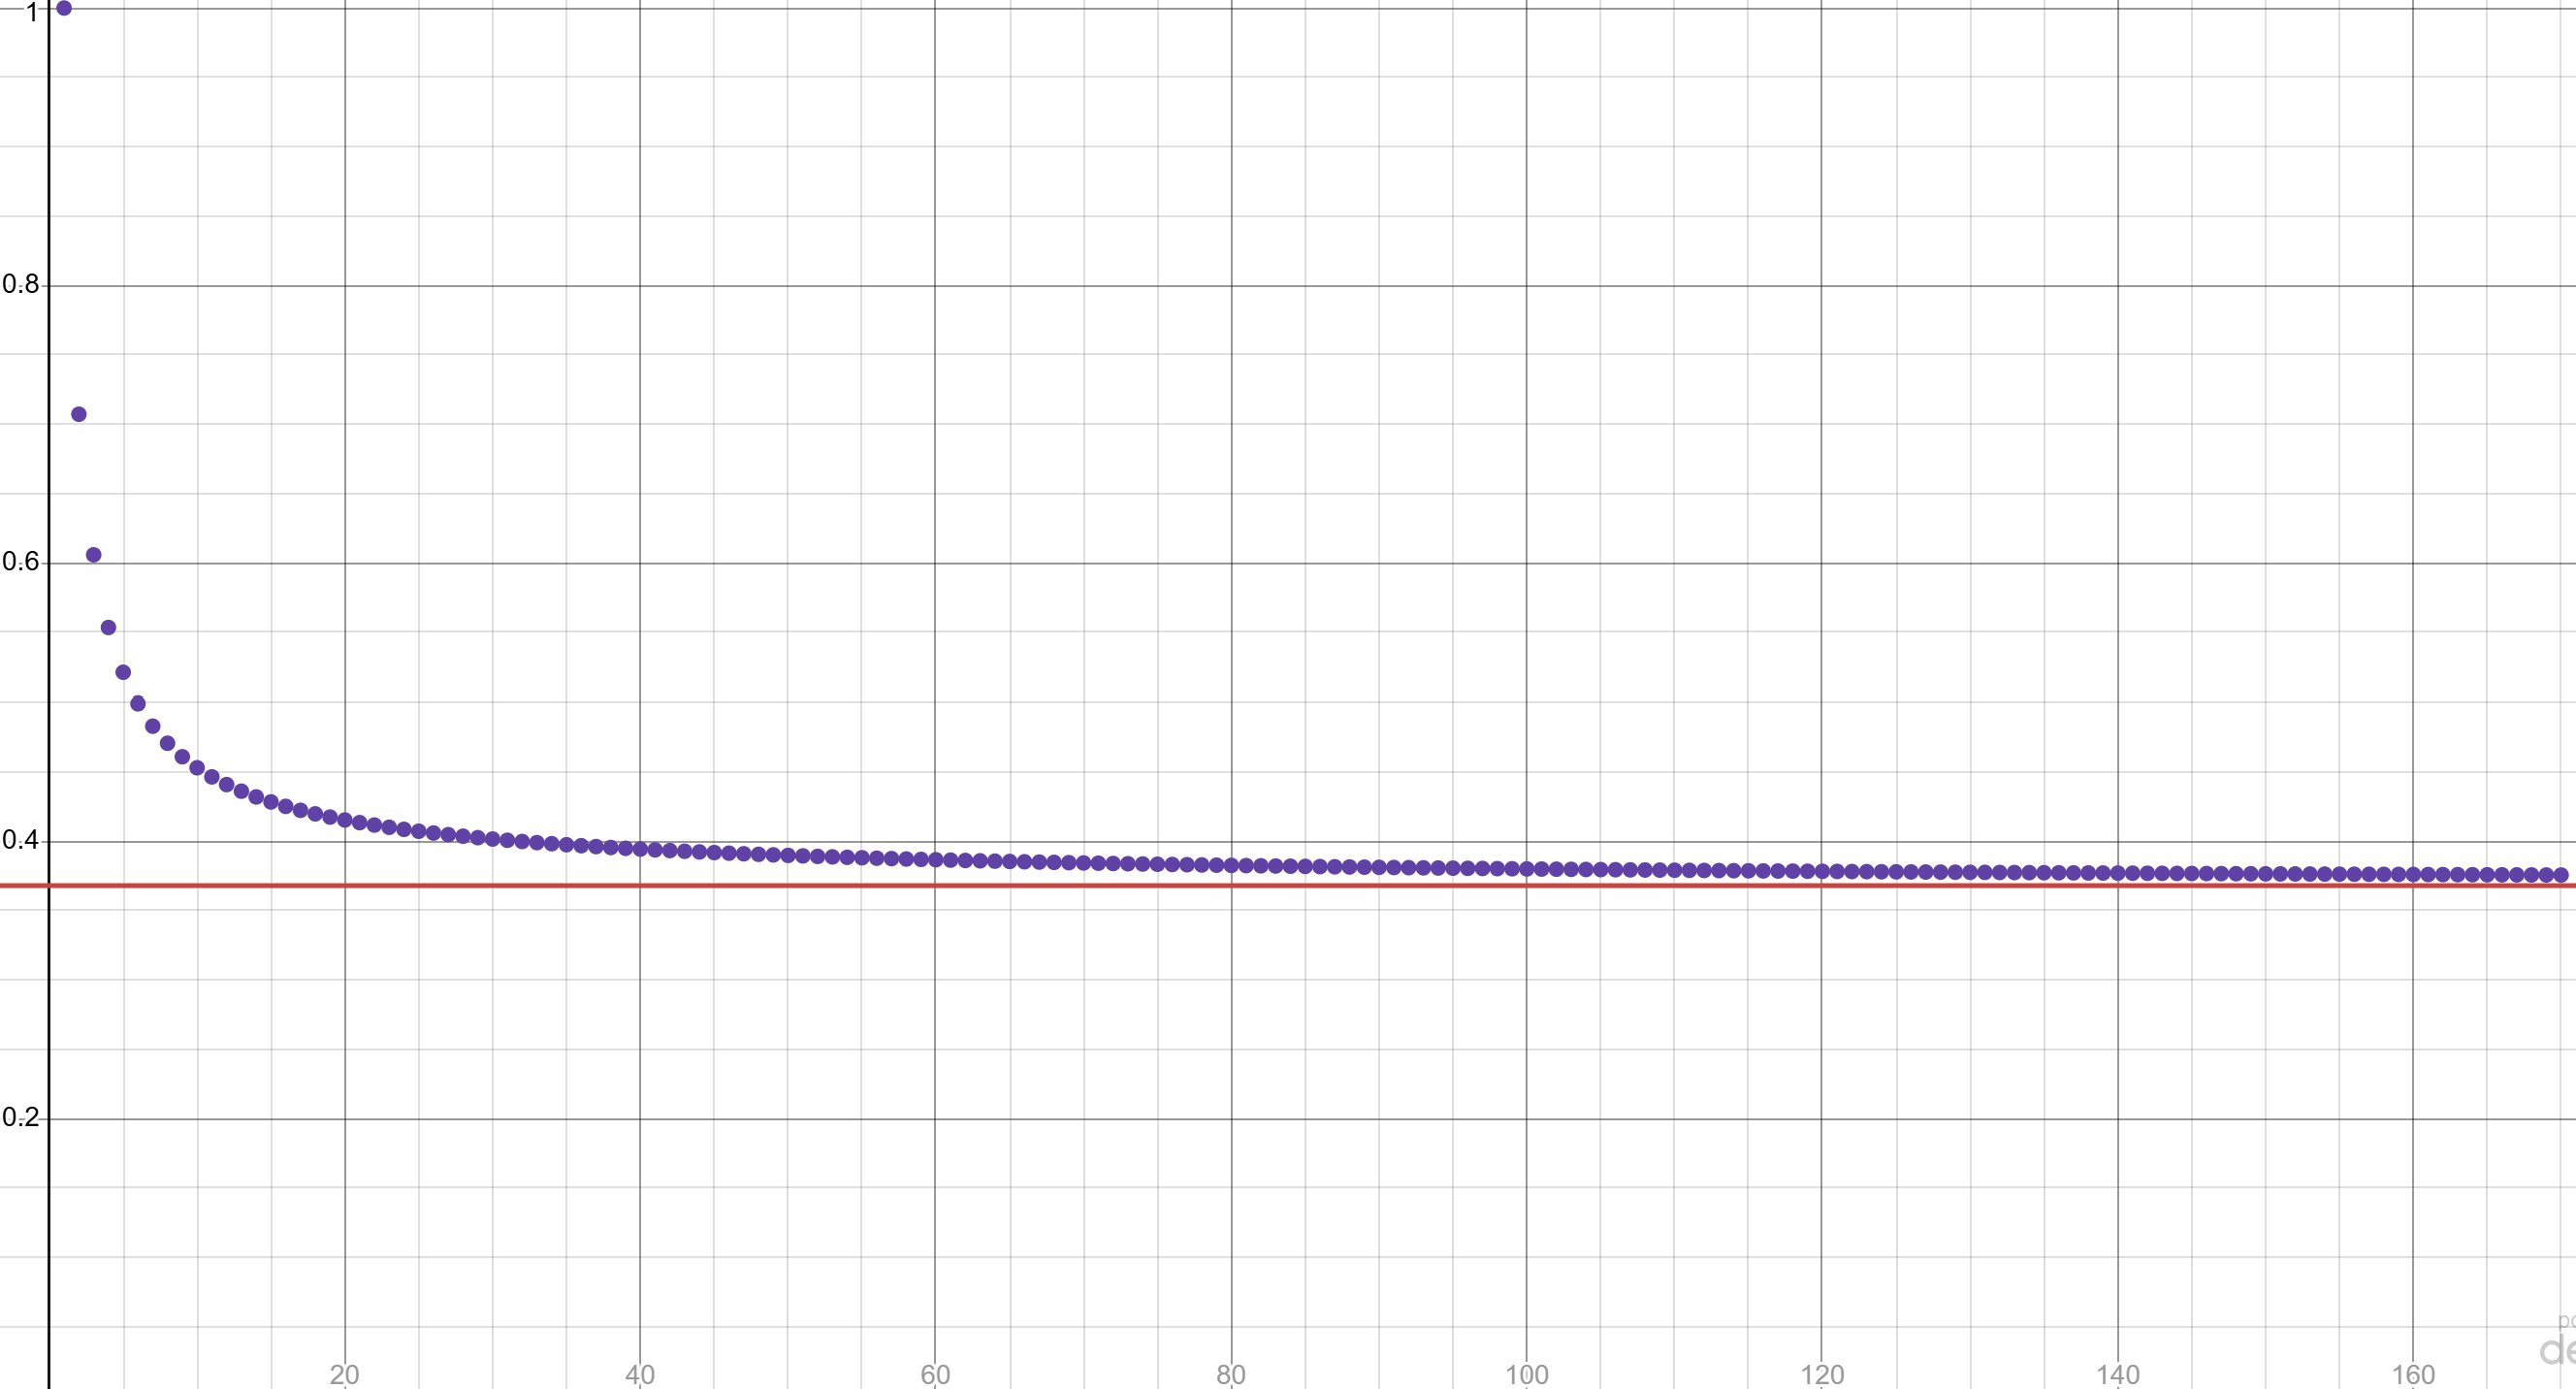
\includegraphics[width=0.8\linewidth]{one_over_e_limit_approach.png}
    \caption{Numerical Verification of the Limit in \eqref{eq:one_over_e_limit}}
\end{figure}
I used a calculator to graph the first 170 points of the equation (the highest the calculator can get), and having a guess of the limit approaches 1/e. This reasonable guessing was taken from the solution in Ratio Test. This led to my 2 conjectures, and it's natural to extend:

1. How does solution 1/e connect to The Optimal Stopping Problem?

2. If the limit exists, how do the limit of Root Test and Ratio Test have the same behavior?
\section{The Optimal Stopping Problem and 1/e}
\subsection{The Optimal Stopping Problem}

When I got the result, I was shocked about the solution, because $1/e \approx 37\%$ occurred in a YouTube video made by the YouTuber Veritasium, which specifically talked about The Optimal Stopping Problem \cite{veritasium_37}.

To illustrate this, we introduce the classical formulation of the Secretary Problem, historically also framed in literature as the \textit{Marriage Problem} (see, e.g., Ferguson \cite{ferguson1989}). Note that this specific setting is adopted solely for clarity and ease of understanding, without any intended bias or targeting. Consider a man who wants to get married within 10 years (from the age of 22 to 32), and he wants to pick the best girl he meets in these ten years. However, he can't go back and pick a girl he met before, meaning he needs to decide whether he is going to marry the girl right at the time or pass. We now want to know what the best strategy is for him to have the highest probability of marrying the best girl.

Let $t \in [22, 32]$ be the time in years. We want to find a stopping point $t_S \in [22, 32]$ to use the following strategy:
\begin{itemize}[itemsep=4pt, topsep=4pt]
    \item When $22 \leq t \leq t_S$, the man only observes the girls to see how good they are. He does not marry anyone in this period.
    \item When $t_S < t \leq 32$, he starts looking for a wife. If he meets a girl who is better than all the girls he met before $t_S$, he marries her immediately.
\end{itemize}

\begin{figure}[H]
\centering
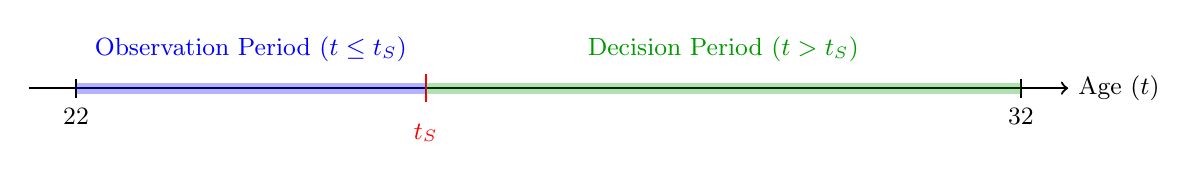
\begin{tikzpicture}[scale=1.2, every node/.style={font=\small}]
    % 画主数轴线
    \draw[thick, ->] (21.5,0) -- (32.5,0) node[right] {Age ($t$)};
    
    % 画刻度线和数字
    \draw[thick] (22,0.1) -- (22,-0.1) node[below] {22};
    \draw[thick] (32,0.1) -- (32,-0.1) node[below] {32};
    \draw[thick, red] (25.7,0.15) -- (25.7,-0.15) node[below=4pt, red] {$t_S$};

    % 用阴影/花括号标记两个不同的区间
    % 1. 观察期 (22 到 S)
    \draw[line width=4pt, blue, opacity=0.3] (22,0) -- (25.7,0);
    \node[above=6pt, blue] at (23.85,0) {Observation Period ($t \leq t_S$)};

    % 2. 决策期 (S 到 32)
    \draw[line width=4pt, green!60!black, opacity=0.3] (25.7,0) -- (32,0);
    \node[above=6pt, green!60!black] at (28.85,0) {Decision Period ($t > t_S$)};

\end{tikzpicture}
\caption{Timeline of the optimal stopping strategy from age 22 to 32.}
\label{fig:stopping_timeline}
\end{figure}

So, our best strategy turns out to be: What $t_S$ can maximize the probability of him to marry the best girl? 

Let's first try some extreme value, that $t_S = 22$ and $t_S = 32$.
\begin{itemize}[itemsep=4pt, topsep=4pt]
    \item $t_S = 22$, he starts to marry at the age of 22, meaning he will {100\%} marry the first girl, because she is the best after S. 
    \item  $t_S = 32$, he is never going to marry until the age of 32. He is forced to pick the last girl and marry. 
\end{itemize}

Obviously those 2 $t_S$ values are the worst, because they are literally equivalent to choose any girl randomly and just to marry.  

To start the proof, we let $N$ be the total number of girls he met in 10 years. 
We assume they appear at a constant rate, so time $t \in [22, 32]$ maps to number $i$ girl by the linear relation:
\[ i(t) = \frac{N}{10}(t - 22) \]

\begin{figure}[H]
\centering
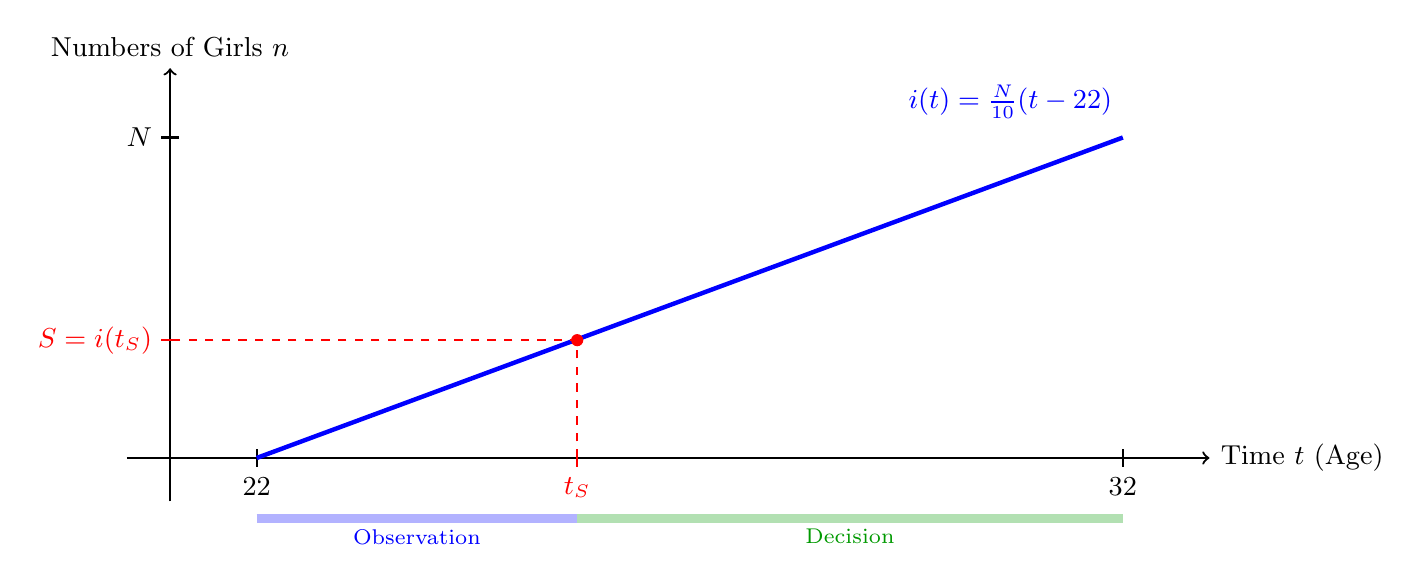
\begin{tikzpicture}[scale=1.1, transform shape, every node/.style={font=\small}]
    % 1. 画坐标轴
    % 横轴：时间 t (从 21.5 画到 33.5，给两头留点余量)
    \draw[thick, ->] (20.5, 0) -- (33, 0) node[right] {Time $t$ (Age)};
    % 纵轴：个体序号 i (从 -0.5 画到 4.5)
    \draw[thick, ->] (21, -0.5) -- (21, 4.5) node[above] {Numbers of Girls $n$};

    % 2. 标出坐标轴的关键刻度
    \draw[thick] (22, 0.1) -- (22, -0.1) node[below] {22};
    \draw[thick] (32, 0.1) -- (32, -0.1) node[below] {32};
    \draw[thick] (20.9, 3.7) -- (21.1, 3.7) node[left=5pt] {$N$};

    % 3. 画线性映射的斜线 (从 (22,0) 连接到 (32,N))
    % 这里用 y=3.7 来代表总数 N
    \draw[ultra thick, blue] (22, 0) -- (32, 3.7);
    \node[blue, above left] at (32, 3.8) {$i(t) = \frac{N}{10}(t - 22)$};

    % 4. 虚线标注临界点 t_S 和 k
    % 假设 t_S 约在 25.7，对应 y 轴上的 k
    \draw[dashed, red, thick] (25.7, 0) -- (25.7, 1.36) -- (21, 1.36);
    
    % 标出红色临界点的刻度
    \draw[thick, red] (25.7, 0.1) -- (25.7, -0.1) node[below] {$t_S$};
    \draw[thick, red] (20.9, 1.36) -- (21.1, 1.36) node[left=5pt] {$S = i(t_S)$};
    \fill[red] (25.7, 1.36) circle (2pt);

    % 5. 区分探索期和决策期（在横轴上加彩色区间条）
    \draw[line width=3pt, opacity=0.3, blue] (22, -0.7) -- (25.7, -0.7);
    \node[below, blue] at (23.85, -0.7) {\scriptsize Observation};
    
    \draw[line width=3pt, opacity=0.3, green!60!black] (25.7, -0.7) -- (32, -0.7);
    \node[below, green!60!black] at (28.85, -0.7) {\scriptsize Decision};
\end{tikzpicture}
\caption{Linear mapping between time $t$ and numbers of girls $n$}
\label{fig:linear_mapping}
\end{figure}
Where we define $S$ be the $S$-th girl he observed, and starts considering to make the decision after $S$.

The probability of ``successfully choose the best option'' can be calculated by adding up all the probabilities ($\sum$) of "successfully choose the nth solution", $\forall n\in \mathbb{N}, S< n \leq N$, so that we can know the probability of getting the best option. For the number nth girl ($S< n \leq N$), we have:

\begin{itemize}[itemsep=4pt, topsep=4pt]
    \item the probability of that girl is the best girl overall: $\frac{1}{N}$
    \item The probability of the strategy successfully chooses the girl: all options k in $S<k\leq n$ is less then the maximum of first S options. Which means we want the best of first $(n-1)$ options is less than $S$. So the probability of that happen is $\frac{S}{n-1}$.
    \item We multiply them, which is the probability of the nth girl is best, and be chosen. 
\end{itemize}
So we add all cases together: 
\begin{align}
    P(\text{successfully choose the best option}) &=\sum_{n=S+1}^{N} \frac{1}{N}\cdot \frac{S}{n-1}\\ 
    &=\frac{S}{N}\sum_{n=S+1}^{N}\frac{1}{n-1} \label{eq:summation_limit_replacement}
\end{align}
Notice that \eqref{eq:summation_limit_replacement} is true because $S$ and $N$ are both constant respect to the summation.
Now, we can change the lower limit and upper limit by substitute $i = n-1$, where $n= i+1$, to rewrite the summation prettier. 
\begin{equation}
    P(\text{successfully choose the best option}) =\frac{S}{N}\sum_{i+1=S+1}^{i+1=N}\frac{1}{i} = \frac{S}{N}\sum_{i=S}^{N-1}\frac{1}{i}
\end{equation}
To deal with the harmonic series easily, we can let $N\to \infty$, and change the series into integral, so we can use the analysis methods. 
\begin{equation}
x_i := \frac{i}{N}, \Delta x := \frac{1}{N} \nonumber
\end{equation}

\begin{align}
    \lim_{N \to \infty} P(\text{successfully choose the best option}) &=\lim_{N \to \infty} \frac{S}{N}\sum_{i=S}^{N-1}\frac{1}{i}\nonumber\\
    &= \lim_{N \to \infty} \frac{S}{N}\sum_{i=S}^{N-1}\frac{1}{\frac{i}{N}\cdot N}\nonumber\\
    &= \lim_{N \to \infty} \frac{S}{N}\sum_{i=S}^{N-1}\frac{1}{i/N}\cdot \frac{1}{N}\nonumber\\
    &= \lim_{N \to \infty} \frac{S}{N}\sum_{i=S}^{N-1}\frac{1}{x_i}\cdot \Delta x \label{eq:riemann_sum}
\end{align}
By considering $S/N$ as $x_S$, we can rewrite the Riemann Sum into a definite integral. Lower bound: $x_S$, Upper bound: $\lim_{N \to \infty} (N-1)/N = 1$
    
\begin{align}
    \eqref{eq:riemann_sum} &=x_S\int_{x=x_S}^{x=1}\frac{1}{x}\cdot  dx \nonumber \\
    &=x\int_{x}^{1}\frac{1}{t} \, dt \nonumber \\
    &=x\left[ \ln{t} \right]_{x}^{1} \nonumber \\
    &=x\left[ \ln{1}-\ln{x} \right] \nonumber \\
    &= -x\ln x
\end{align}
This is the function of x where x is the ratio of stopping point $S$ and total number $N$, when $N$ approaches infinity. This is the ultimate probability of choose the best girl. 

So, we want to maximize the function, to find the best value of $S/N$. 

\begin{align}
    \frac{dy}{dx}=0 \iff\frac{dy}{dx} &= \frac{d}{dx}(-x\ln x)\nonumber\\
    &= -\ln x +(-1)=0 \nonumber\\
    \implies -\ln x = 1 \implies \ln x = -1 \implies x= e^{-1}=1/e
\end{align}
At the point where the ratio of $S$ and $N$ are $1/e$, there is a highest probability of ``successfully choose the best girl". For example, in this scenario, the best $t_S$ is $22+10/e \approx 25.7$ years.

We can notice that this ratio is equal to the limit we discovered before: $\lim_{n \to \infty} \frac{\sqrt[n]{n!}}{n}$ \eqref{eq:one_over_e_limit} 

\subsection{Connections of 1/e}

Let's rewrite the equations:
\begin{equation}
    \lim_{n \to \infty} \frac{\sqrt[n]{n!}}{n}= \frac{S}{N}=\frac{1}{e}
\end{equation}
We want to see what is the connections. 
\bibliographystyle{plain}
\bibliography{references}
\end{document}
